\documentclass{article}
\usepackage[a4paper,top=2.5cm,bottom=2.5cm,left=2.5cm,right=2.5cm]{geometry}
\usepackage{makeidx}
\usepackage{graphicx}
\usepackage{listings}
\usepackage{color}
\usepackage[table]{xcolor}
\usepackage{alltt}
\usepackage{ifpdf}
\ifpdf
\usepackage[pdftex,
            pagebackref=true,
            colorlinks=true,
            linkcolor=black,
            unicode
           ]{hyperref}
\else
\usepackage[ps2pdf,
            pagebackref=true,
            colorlinks=true,
            linkcolor=black,
            unicode
           ]{hyperref}
\usepackage{pspicture}
\fi
\usepackage[utf8]{inputenc}
%\usepackage{mathptmx}
\usepackage[scaled=.90]{helvet}
\usepackage{courier}
\usepackage{sectsty}
%\usepackage{amssymb}
\usepackage[titles]{tocloft}
%\usepackage{doxygen}
\lstset{language=C++,inputencoding=utf8,basicstyle=\footnotesize,breaklines=true,breakatwhitespace=true,tabsize=8,numbers=left }
\lstset{language=XML,inputencoding=utf8,basicstyle=\footnotesize,breaklines=true,breakatwhitespace=true,tabsize=8,numbers=left,keywordstyle=\color{blue},morekeywords={profile,modules,launcher},numberstyle=\tiny\color{gray}, backgroundcolor=\color{gray}}
\lstset{language=bash,inputencoding=utf8,basicstyle=\footnotesize,breaklines=true,breakatwhitespace=true,tabsize=8 }

\makeindex
\setcounter{tocdepth}{3}
%\renewcommand{\footrulewidth}{0.4pt}
\renewcommand{\familydefault}{\sfdefault}
\hfuzz=15pt
\setlength{\emergencystretch}{15pt}
\hbadness=750
\tolerance=750

\author{Sogeti High Tech}
\title{Runtime Configuration for MPC - Developper Manual}
\date{\today}

\begin{document}
\hypersetup{pageanchor=false,citecolor=blue}
\maketitle

\newpage
\pagenumbering{roman}
\tableofcontents
\newpage
\pagenumbering{arabic}
\hypersetup{pageanchor=true,citecolor=blue}

\section{Introduction}

Since MPC 2.4.1, a configuration system has been introduced through the module \texttt{MPC\_Config}: it enables the user to setup some parameters at the runtime when running his binary with MPC.
\newline

\noindent This manual will explain to a developper how the configuration system is designed and how to add parameter into it.

\section{The module MPC\_Config}

All the configuration system is implemented into the \texttt{MPC\_Config} module which gives functionnalities to generate:
\begin{itemize}
\item The configuration structure;
\item The UNIX man for options list and values;
\item The parsing source code;
\item The displaying function.
\end{itemize}

\noindent This module also contains the graphical editor sources.

\newpage

\section{Sources of the modules MPC\_Config}

The module \texttt{MPC\_Config} is subdivided into several directories:
\begin{itemize}
\item \texttt{bin}: contains the sources of the \texttt{mpc\_print\_config} executable;
\item \texttt{doc}: contains the user and developper manuals describing the configuration system;
\item \texttt{editor}: contains the graphical configuration editor;
\item \texttt{generated}: contains all the generated files needed at the runtime (see §\ref{conf_gen_config} for more details);
\item \texttt{generators}: contains all XSLT files used to generate the files in the \texttt{generated} folder;
\item \texttt{src}: contains the sources for the configuration parsor from XML files (see §\ref{conf_src_config} for more details).
\end{itemize}

\subsection{Details for the editor folder}
\label{conf_editor_config}
The \texttt{editor} folder contains:
\begin{itemize}
\item \texttt{config}: contains a set of different configs (valid, unvalid and malformed) which can be used as example for the editor;
\item \texttt{images}: contains all the images used in the editor;
\item \texttt{javascript}: contains all the JavaScript scripts used to load and edit configuration files;
\item \texttt{style}: contains all the CSS files defining the editor style;
\item \texttt{index.html}: the main file to open in a browser to use the graphical editor.
\end{itemize}

\subsection{Details for the generated folder}
\label{conf_gen_config}
Several files are generated using the XSLT in the \texttt{generators} folder:
\begin{itemize}
\item \texttt{sctk\_runtime\_config\_struct.h}: define all the C data structures (\texttt{struct}, \texttt{enum}, etc.) of the MPC configuration structure;
\item \texttt{sctk\_runtime\_config\_struct\_meta.c}: define meta-description (datatype, offset into the structure, etc.) to load the MPC configuration structure;
\item \texttt{sctk\_runtime\_config\_struct\_defaults.h}: define functions prototypes initializing the MPC configuration structure with the default values;
\item \texttt{sctk\_runtime\_config\_struct\_defaults.c}: initialize the MPC configuration structure with the default values;
\item \texttt{global-config-meta.xml}: contains the contents of each \texttt{config-meta.xml} existing in MPC;
\item \texttt{mpc\_config.5}: UNIX man describing all the parameters (type, default value, doc) of the MPC configuration structure;
\item \texttt{mpc-config.xsd}: scheme to validate the final configuration file.
\end{itemize}

\subsection{Details for the src folder}
\label{conf_src_config}

The \texttt{src} folder contains the following files:
\begin{itemize}
\item \texttt{sctk\_runtime\_config\_mapper.\{.h,.c\}}: provide the functions to convert the XML configuration file to the C structure;
\item \texttt{sctk\_runtime\_config\_printer.\{.h,.c\}}: use by the \texttt{mpc\_print\_config} executable to display the parameters for the XML configuration file, using the file \texttt{sctk\_runtime\_config\_struct\_meta.c};
\item \texttt{sctk\_runtime\_config\_selectors.\{.h,.c\}}: handle selectors to select dynamically profiles at execution time;
\item \texttt{sctk\_runtime\_config\_sources.\{.h,.c\}}: provide the functions to open XML configuration files and to select profiles to apply;
\item \texttt{sctk\_runtime\_config\_validation.\{.h,.c\}}: provide a function to overwrite parameters with environment variables, and a function to check the values of the parameters;
\item \texttt{sctk\_runtime\_config\_walk.\{.h,.c\}}: use to run over the C configruation structure in order to display its contents;
\item \texttt{sctk\_runtime\_config.\{.h,.c\}}: provide the interface that will be used in the other MPC modules.
\end{itemize}

\noindent A module \texttt{sctk\_libxml\_helper.\{.h, .c\}} is also developped to use \texttt{libxml2} to read and write XML files.

\section{The configuration system into MPC}

\subsection{Write a \texttt{config-meta.xml} file}

Each module to be added in the configuration system needs its own \texttt{config-meta.xml} file. The general structure of such a file is designed as follow:

\lstset{language=XML}
\begin{lstlisting}[title=General structure of a \texttt{config-meta.xml} file]
<config>
  <usertypes>...</usertypes>
  <modules>...</modules>
<profile>
\end{lstlisting}

\noindent The developer has to defined all the types (\texttt{structure}, \texttt{union}, etc.) that will be used into the configuration system in the \texttt{usertypes} section.

\subsubsection{The \texttt{usertypes} section}

In this section, the developer will define structures (\texttt{struct}), unions (\texttt{union}) and enumerators (\texttt{enum}) that will be used in the configuration system. Each one of them have two required attributes:
\texttt{name} (resp. \texttt{doc}) is the name (resp. the description) of the variable/object.
\newline

\noindent A structure (as a C/C++ struct) is a set of \texttt{param} or \texttt{array} which have required attributes:
\begin{enumerate}
\item \texttt{name} which is the name of the variable;
\item \texttt{type} which is its type (simple: \texttt{int}, \texttt{float}, \dots or complex: \texttt{struct}, \texttt{union}, \dots),
\item \texttt{doc} which shortly describes what it is for,
\item \verb![!only for \texttt{array}\verb!]! \texttt{entry-name} which matches to the tag name of the array elements.
\end{enumerate}

\noindent The \texttt{param} have an optional attribute, \texttt{default}, to initialize the variable to a specific default value.

\lstset{language=XML}
\begin{lstlisting}[title=Example of a \texttt{struct} definition]
<struct name="my_struct" doc="This a struct test">
  <param name="param1" type="string" doc="String param." />
  <param name="param2" type="user_type" doc="Param of type user_type (enum, struct, ...)." />
  <array name="array1" entry-name="elt" type="int" doc="Array of int with elt as xml tag name." />
</struct>
\end{lstlisting}

\noindent An union (as a C/C++ union) matches to a list of choices defined by a name and a type.

\lstset{language=XML}
\begin{lstlisting}[title=Example of a \texttt{union} definition]
<union name="my_union" doc="This an union test">
  <!-- Define a choice with a string param -->
  <choice name="choice1" type="string" />
  <!-- Define a choice with an user type param -->
  <choice name="choice2" type="user_type" />
  <!-- Define a choice with an int param -->
  <choice name="choice3" type="int" />
</union>
\end{lstlisting}

\noindent An enumerator (as a C/C++ enum) is a set of possible values as shown in the following code.

\lstset{language=XML}
\begin{lstlisting}[title=Example of a \texttt{enum} definition]
<enum name="day" doc="Week days">
  <value>Monday</value>
  <value>Tuesday</value>
  <value>Wednesday</value>
</enum>
\end{lstlisting}

\subsubsection{The \texttt{modules} section}

In this section, the developer will declare the high-level structures he wants the user to configure. In the following code, there will be two configurable structures of type \texttt{my\_struct\_1} and
\texttt{my\_struct\_2}.

\lstset{language=XML}
\begin{lstlisting}[title=Example of a \texttt{modules} definition]
<modules>
  <module name="struct_1" type="my_struct_1" />
  <module name="struct_2" type="my_struct_2" />
</modules>
\end{lstlisting}

\subsection{Configuration management workflow}

The workflow of configuration management can be described by steps:
\begin{enumerate}
\item Write a \texttt{config-meta.xml} for each MPC module which needs to be integrated into the configuration system;
\item Run \texttt{mpc\_gen\_runtime\_config} which will :
\begin{itemize}
\item Aggregate all the \texttt{config-meta.xml} to generate the \texttt{global-config-meta.xml};
\item Apply XSLT transformations to generate source code for configuration management;
\end{itemize}
\item Compile MPC;
\end{enumerate}

\noindent The Figure ~\ref{fig:conf_workflow_conf} summarized this process.

\begin{figure}[htc!]
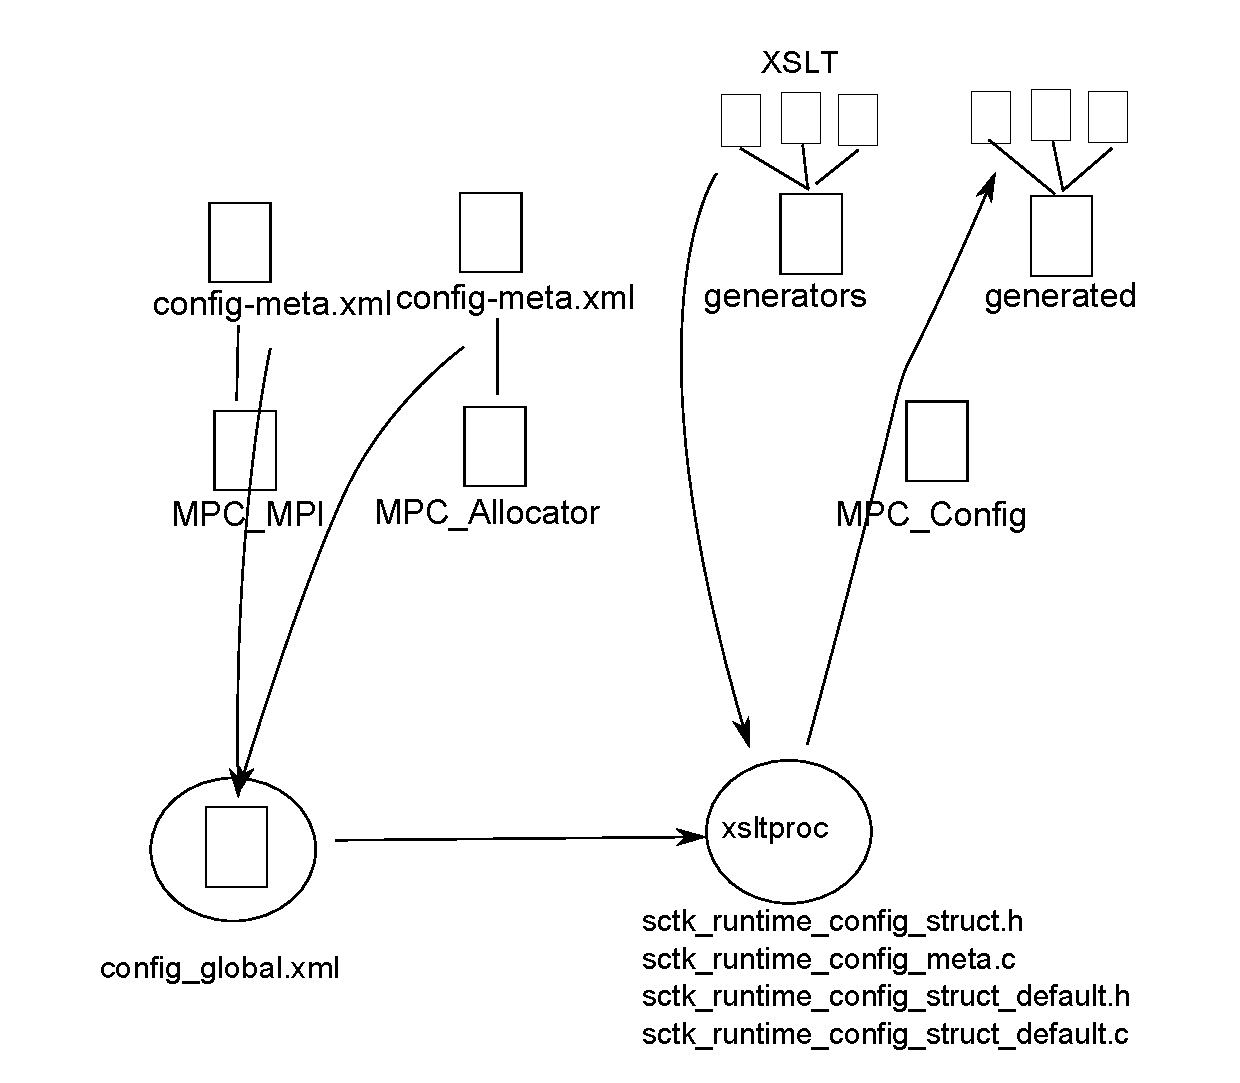
\includegraphics[scale=0.8]{file-workflow.pdf}
\caption{Representation of the workflow}
\label{fig:conf_workflow_conf}
\end{figure}

\subsection {Steps for developper}

A developper who wants to integrate his MPC module into the configuration system must:
\begin{enumerate}
\item Create a configuration file \texttt{config-meta.xml} in his module and define all the options he wants to parametrized;
\item Mark the dependency to the MPC\_Config module by adding in the file \texttt{module\_dep}: \texttt{need\_module MPC\_Config};
\item Regenerate the MPC\_Config auto-generated files by execution \texttt{./MPC\_Tools/mpc\_gen\_runtime\_config} from \texttt{mpc} directory;
\item Include the header \texttt{sctk\_runtime\_config.h} in his source files;
\item Use the function \texttt{sctk\_runtime\_config\_get()} to access to the configuration structure.
\end{enumerate}

\newpage

\section{The graphical editor interface}

To edit the generated configuration files, an editor has been developed in HTML/JavaScript. The development has been validated on Firefox 10.0.8 ESR, but works with several others browsers as Google Chrome or Safari.
\newline

\noindent This section will only describe the JavaScript sources. In order to make future evolutions easy, the code is organized in a Model-View-Controller pattern. The model represents the data read from the XML configuration file: it is an association of hash tables which store propeties informations (name, type, value(s), etc.). The view is the graphical representation of the model, and the controller manages the events to synchronize both the model and the view.

\noindent Some extra libraries have been included:
\begin{itemize}
\item \texttt{EditorXML.js} to manage the XML: conversion functions, getting child nodes, etc.;
\item \texttt{xmllint.js} is a module compiled from libxml, which is used to validated the XML files (data and structure speaking);
\item \texttt{BlobBuilder.js} and \texttt{FileSaver.js} to handle the saving of the new XML generated file.
\end{itemize}

\subsection{The model}

The model is handled in the \texttt{EditorModel.js} which can be separated in several parts:
\begin{itemize}
\item The functions used to create the model from an XML file;
\item The functions used to update the model;
\item The functions used to generate an XML file from the model.
\end{itemize}

\noindent A configuration file is divided in three parts, and each one has its own generation function:
\begin{enumerate}
\item The \texttt{profiles} section is generated by \texttt{createProfilesModel(config)};
\item The \texttt{networks} section is generated by \texttt{createNetworksModel(config)};
\item The \texttt{mappings} section is generated by \texttt{createMappingsModel(config)}.
\end{enumerate}
\noindent where \texttt{config} matches to the XML read configuration file converted into an DOM Document HTML Object.
\newline

\noindent The model generation has been thinked in such a way that it is fully  automatic. While the XML configuration file is reading, the functions reads in the \texttt{sctk\_runtime\_config\_meta.js} (which is a conversion of \texttt{sctk\_runtime\_config\_meta.h} generated with XSL in JavaScript format) to get the type of each property. Depending on its type (\texttt{param}, \texttt{array}, \texttt{struct}, \texttt{union}), the model of a property is generated with one of the following functions:
\begin{itemize}
\item \texttt{createStructModel(xml, js)};
\item \texttt{createArrayModel(xml, js)};
\item \texttt{createParamModel(xml, js)};
\item \texttt{createUnionModel(xml, js)};
\end{itemize}
where \texttt{xml} matches to the property read in the XML configuration file and \texttt{js} is its meta-information.
\newline

\noindent If a new type called \texttt{XXX} is inserted in the configuration system, the developer just has to developed a function \texttt{create\textit{XXX}Model(xml, js)} to create the associated model for a given property.
\newline

\noindent \texttt{EditorModel.js} also provides functions to update the model when a property value has been changed in the editor. Here is a list of some available functions:
\begin{itemize}
\item \texttt{updateModel} to update a module value in a profile;
\item \texttt{upateMappingsModel} to update the mappings section;
\item etc.
\end{itemize}

\noindent Finally, this file contains the XML generation functions. Each part of the configuration file has its own, and each type too. In this way, the XML generation is fully automatic:
\begin{itemize}
\item \texttt{generateMappingsXmlConfig} to generate the XML code for the mappings section;
\item \texttt{generateStructXML} for a property of \texttt{struct} type;
\item \texttt{generateParamXML} for a property of \texttt{param} type;
\item etc.
\end{itemize}

\subsection{The view}

The view is handled in the \texttt{EditorView.js} which is also divided in several parts:
\begin{itemize}
\item The functions used to create the view from the model;
\item The functions used to update the view when the model is updated.
\end{itemize}

\noindent As for the model, a generation function is developed for each part of a configuration file:
\begin{enumerate}
\item The \texttt{profiles} section is generated by \texttt{createProfilesView};
\item The \texttt{networks} section is generated by \texttt{createNetworksView};
\item The \texttt{mappings} section is generated by \texttt{createMappingsView}.
\end{enumerate}

\noindent Each property type has its own function to create its representation:
\begin{itemize}
\item Numbers, function pointers and strings will be drawn an input text;
\item Enumerators are represented with combo box;
\item Sizes are an association between an input text and a combo box.
\end{itemize}

\subsection{The controller}

The file \texttt{EditorController.js} gives functionnalities to manage editor events to synchronize the model and the view.
\begin{itemize}
\item Adding/deleting new elements (profiles, mappings, etc.);
\item Property updating;
\item etc.
\end{itemize}

\subsection{The XML handling}

The file \texttt{EditorXML.js} implements some functions to manage XML files.
\newline

\noindent The \texttt{StringToXML} (resp. \texttt{XMLToString}) converts an XML document into a string (resp. a string to an XML document). \texttt{formatXML} formats a XML code to respect indentation tags.
\newline

\noindent XML parsing functions are also implemented:
\begin{itemize}
\item \texttt{getNodes} gets all the XML elements matching to a given name;
\item \texttt{hasChild} returns the child of a given XML element;
\item \texttt{getChildNodes} returns all the child of a given XML element;
\item \texttt{getNodeValue} returns the text value of a given XML element.
\end{itemize}

\noindent To ensure the portability of the editor, the \texttt{getElementsByClassName} has been recoded: it returns all the XML elements of a given node (the entire document by default) matching to a class name.

\subsection{Opening and saving local files}

JavaScript forbids to open and save local files for security reasons.
\newline

\noindent However, the module \texttt{FileReader} (new in HTML5) lets the user to open local files. Events are associated to this class:
\begin{itemize}
\item \texttt{onload} is triggered at the end of the file reading. Once the content loaded, it is analyzed by \texttt{xmllint.js} and the associated XSD file to validate its consistency. If the XML file is not valid, it will not be opened, and an error message will be displayed. Otherwise, the file will be loaded.
\item \texttt{onerror} is triggered when an error occurs during the file reading. If this event is catched, the XML file will not be loaded.
\end{itemize}

\noindent To save files on a local disk storage, classes \texttt{BlobBuilder.js} and \texttt{FileSaver.js} have been added to the editor.
\end{document}
